
\begin{figure}[h!]
    \centering
    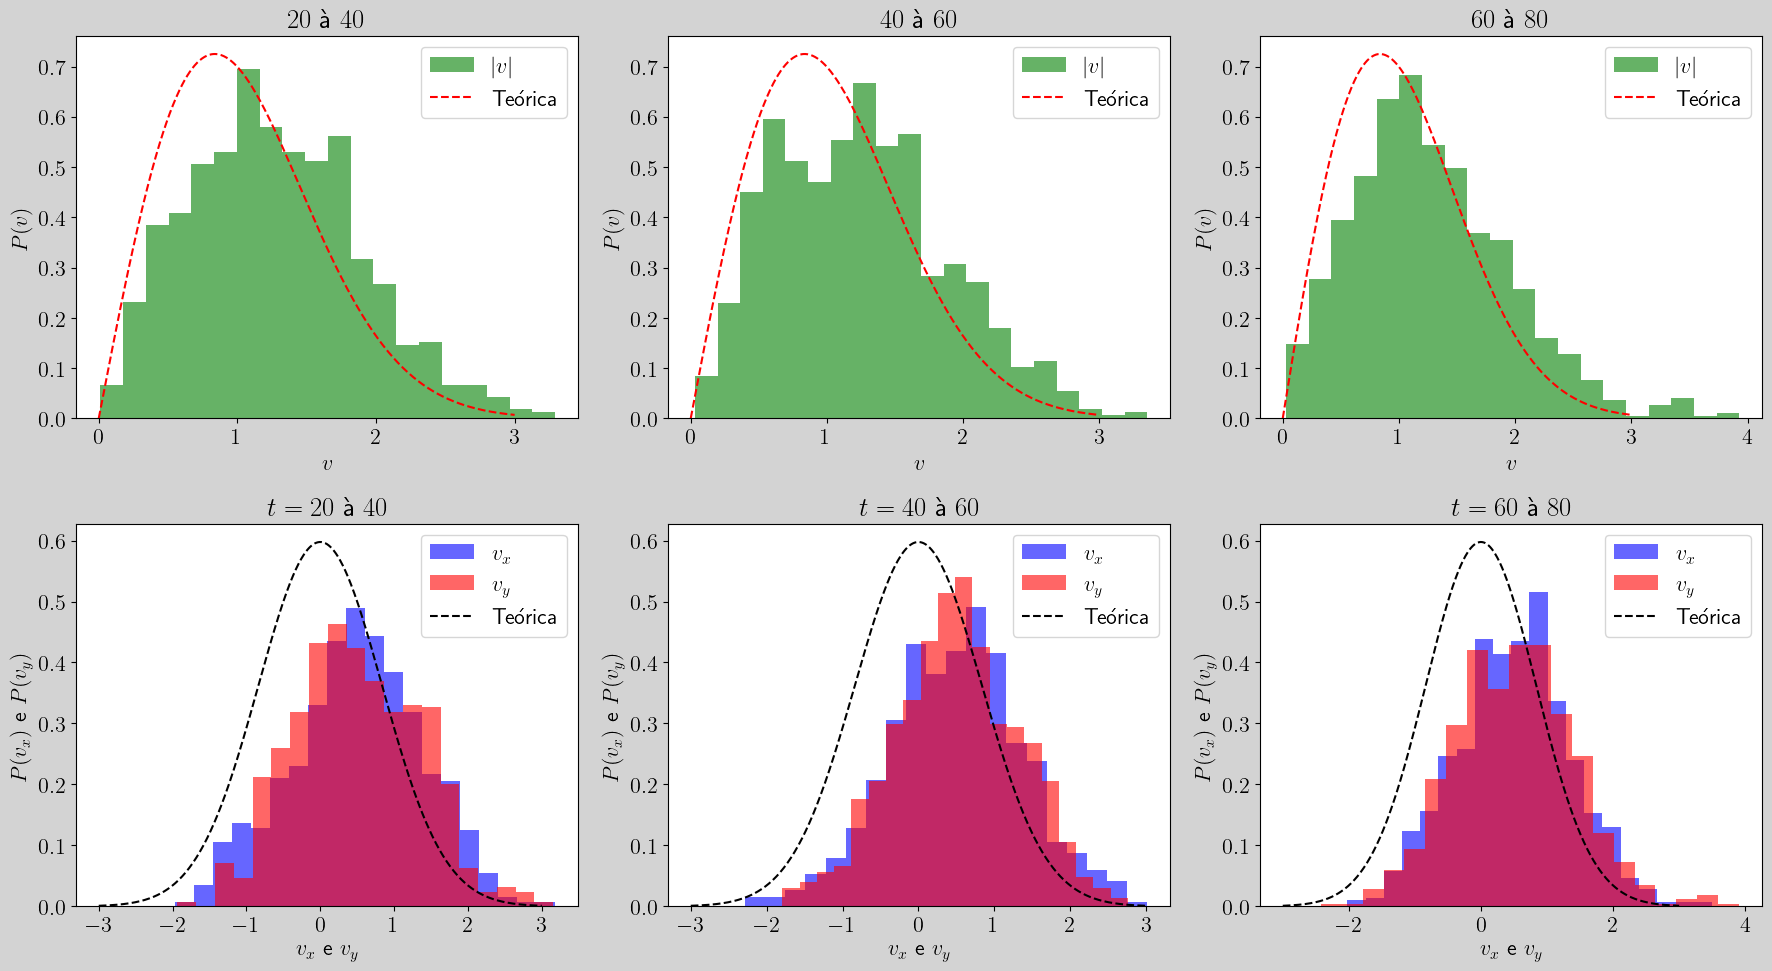
\includegraphics[width=0.7\linewidth]{tarefa-C/distribuicoes-c.png}
    \caption{Distribuição da velocidade, magnitude e componentes em intervalos $t=20-40$, $t=40-60$ e $t=60-80$.}
    \label{fig:distribuicoes-velocidade-c}
\end{figure}



\subsection*{Código}
Nesse código temos a simulação desse item, considerandos as mudanças do perfil inicial de velocidades 
das partículas. E além disso ela também gera os dados necessários para o cálculo da tarefa posterior, D, assim 
como parte do código da tarefa A também fazia o mesmo.
\begin{minted}{fortran}

    ! Tarefa C
    implicit real*8(a-h, o-y)
    parameter (pi = acos(-1.e0))
    dimension r_prev(20, 2)
    dimension r_curr(20, 2)
    dimension r_next(20, 2)
    dimension v(20, 2)
    dimension acc(2)
    dimension r(20, 20)
    L = 10
    rL = 10d0
    N = 20
    dt = 0.02
    v0 = 1.0

    open(unit = 7,  file="saidas/tarefa-C/velocidades.dat")
    open(unit = 4,  file="saidas/tarefa-C/evolucao-posicoes.dat")
    open(unit = 66, file="saidas/tarefa-C/velocidades-iniciais.dat")

    ! Tarefa D
    open(unit = 8,  file="saidas/tarefa-D/temperatura-c.dat")
    ! Modificacoes para tarefa C

    r_prev = 0 
    r_curr = 0 
    r_next = 0
    acc = 0 

    ! Setting velocities 
    v = 0 
    do i = 1, N/2
          v(i, 1) = v0
          v(i+N/2, 2) = v0
    end do

    ! Initialize particles 

    n_cols = ceiling(sqrt(N*1d0))
    n_rows = ceiling((N*1d0)/(n_cols*1d0)) 

    ! Spacing 1/4 
    x_spacing = L/(1d0*n_cols)
    y_spacing = L/(1d0*n_rows)

    spacing = min(x_spacing, y_spacing)/4.0 

    ! Centering in the grid
    x_offset = x_spacing / 2.0 
    y_offset = y_spacing / 2.0

    call srand(124689)

    k = 1 
    do j = 1, n_rows 
          do i = 1, n_cols 
                r_curr(k, 1) = (i-1)*x_spacing+x_offset
                r_curr(k, 2) = (j-1)*y_spacing+y_offset

                r_curr(k, 1) = r_curr(k,1)+(rand())*spacing
                r_curr(k, 2) = r_curr(k,2)+(rand())*spacing

                r_prev(k, 1) = r_curr(k, 1) - v(k, 1) * dt 
                r_prev(k, 2) = r_curr(k, 2) - v(k, 2) * dt 
                k=k+1
          end do 
    end do

    ! Dynamics 
    do k = 1, 5000

          t = k * dt 
          acc(1) = 0d0 
          acc(2) = 0d0
          do i = 1, N 
                acc(1) = 0d0 
                acc(2) = 0d0

                do j = 1, N 
                      if(i /= j) then
                           call compute_acc(N,i,j,L,r_curr,acc, r)
                      end if
                end do 

                ! UPDATE POSITIONS
                r_next(i,1) = 2*r_curr(i,1)-r_prev(i,1)+acc(1)*(dt**2)
                r_next(i,2) = 2*r_curr(i,2)-r_prev(i,2)+acc(2)*(dt**2)      

                r_next(i,1) = mod(r_next(i,1)+rL, rL)
                r_next(i,2) = mod(r_next(i,2)+rL, rL)

                delta_r_x = delta_pbc(r_next(i,1),r_prev(i,1),L)
                delta_r_y = delta_pbc(r_next(i,2),r_prev(i,2),L)
                ! UPDATE VELOCITIES using adjusted displacements
                v(i, 1) = delta_r_x / (2 * dt)
                v(i, 2) = delta_r_y / (2 * dt)
          end do

          ! SWAP VECTOR POSITIONS.
          r_prev(:, 1) = r_curr(:, 1)
          r_prev(:, 2) = r_curr(:, 2)

          r_curr(:, 1) = r_next(:, 1)
          r_curr(:, 2) = r_next(:, 2)

          if(mod(k, 20) == 0) then
                do i = 1, N
                      v_mag = sqrt(v(i,1)**2+v(i,2)**2)
                      write(7,*) k,  v_mag, v(i,1), v(i,2)
                      write(8,*) .5d0 * v_mag**2
                      write(4,*) k, r_curr(i,1),r_curr(i, 2)
                end do
          end if
    end do
    close(4)
    close(8)
    end 

    function delta_pbc(r_next, r_prev,L)
          implicit real*8(a-h, o-y)
          delta_pbc = r_next - r_prev
          delta_pbc = delta_pbc - L * nint(delta_pbc / L)
    end function delta_pbc



    ! Updates acceleration a = ax, ay 
    ! between particle i and all others
    subroutine compute_acc(N,i,j,L,r_curr,acc, r)
          implicit real*8(a-h, o-y)
          dimension r_curr(20, 2)
          dimension acc(2)
          dimension r(20, 20)
          epsilon = 1e-3

          dx = r_curr(i, 1) - r_curr(j, 1)
          dy = r_curr(i, 2) - r_curr(j, 2)

          dx = dx - L * nint(dx / L)
          dy = dy - L * nint(dy / L)

          r_ij = sqrt(dx**2 + dy**2)

          r(i, j) = r_ij 
          r(j, i) = r_ij

          if(r_ij > epsilon .and. r_ij <= 3d0) then 
                F = 24.0 * (2d0/r_ij**13 - 1d0/r_ij**7)
                acc(1) = acc(1) + F * dx / r_ij 
                acc(2) = acc(2) + F * dy / r_ij
          end if 
    end subroutine compute_acc

    subroutine compute_energy(N, L, v, r_curr, E, r)
          implicit real*8(a-h, o-y)
          dimension v(20, 2)
          dimension r_curr(20, 2)
          dimension r(20, 20)

          epsilon = 1e-3
          Tk = 0d0
          do i = 1, N
              Tk = Tk + 0.5 * (v(i, 1)**2 + v(i, 2)**2)
          end do
          U = 0d0
          do i = 1, N
            do j = i + 1, N
                r_ij = r(i, j)

                if (r_ij > epsilon .and. r_ij <= 3d0) then
                    U = U + 4 * (r_ij**(-12) - r_ij**(-6))
                end if
            end do
          end do
          E = Tk + U
    end subroutine
\end{minted}
\clearpage